\documentclass[a4paper]{article}

\usepackage[margin=0.5cm]{geometry}
\usepackage{qtree}
\usepackage{color}
\usepackage{forest}
\usepackage{tikz}
\usepackage{listings}

\begin{document}
\begin{titlepage}
	\begin{center}
		\begin{figure}[t]
			\centering
			
\includegraphics[width=350px]{logo.PNG}
		\end{figure}
		
		\begin{center}
			\textsc{\Huge Programming Languages}
		\end{center}
		\begin{center}
			\textsc{\Huge COS 333}
		\end{center}
		\begin{center}		
			\textsc{\LARGE Practical Lab Experience 1:}		
		\end{center}
		\begin{center}		
			\textsc{\LARGE Research Assignment}		
		\end{center}
		
		\begin{flushright} \large
			Juan Jaques du Preez \newline \emph{u15189016} \newline
		\end{flushright}
\par\vspace{\fill}
{\large Date:}
\\
{\large \today}

	\end{center}
\end{titlepage}

\tableofcontents
\newpage

\section{Overview}
	\subsection{Overall UML Diagram}
		\begin{center}
			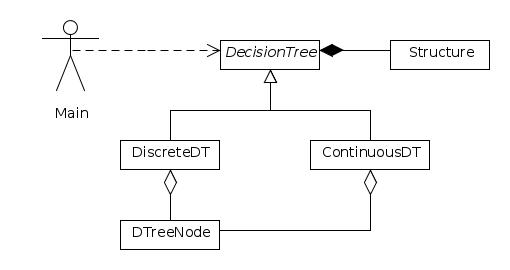
\includegraphics[width=350px]{overview.jpg}	
		\end{center}
		
	\subsection{Options Implemented}
	\begin{itemize}
	\item -d
	\item -c
	\item -md
	\item not -mc
	\item -pd
	\item some of -pc
	\end{itemize}		
	
	\subsection{Please Note}
	The code is not as efficient as it could be. For example, I have two functions in DiscreteDT called induceWithMissing() and induceNoMissing(). These two are very much the same, but I wanted to make the different algorithms that were used as clear as possible.
\section{Compile and Run Program}
For this project I used the language of C++.
	\subsection{Compile}
	To compile the program, open a terminal and type in the following commands:
	\newline
	\newline
	\textbf{cd DecisionTree/} \newline
	\textbf{make} 
	\newline
	\newline
	The makefile compiles the .h and .cpp files into a "runnable" file in the TestSpace/ directory.
	
	\subsection{Run}
	To run the program, make sure you are in the "TestSpace/" directory. Copy the two files (data file and spec file) into 			this directory. Open a terminal and type: \newline
	\newline	
	\textbf{./DecisionTree  option specfile datafile}
	\newline	
	\newline
	Where option is one of: -d, -c, -md, -mc, -pd, -pc.
	
	
	\subsection{Contact}
	If you cannot get the program to compile and run, or have any other issue with regards to anything, please contact me: \newline
	Juan du Preez\newline
	078 141 0915\newline
	u15189016@tuks.co.za\newline
	juan.dupreez82@gmail.com
	
	\subsection{What does not work}
	To make your job easier, here is a list of things that do not work: \newline
	\begin{itemize}
	\item There is no implementation for missing values when doing continuous data with missing values, i.e. the -mc option.
	\item The -pc option, or pruning the tree for continuous data, sometimes goes into an infinite loop. 
	\end{itemize}
	
	
\end{document}
